\chapter{Giới thiệu}
\label{Chapter1}

Chương này trình bày bối cảnh, vấn đề nghiên cứu và phạm vi của bài toán phân lớp ảnh X-quang xương bằng học sâu đa phương thức. Trọng tâm của khóa luận là khai thác đồng thời ảnh X-quang và nguồn văn bản đi kèm. Khóa luận áp dụng hai kịch bản dữ liệu gồm nguồn văn bản chính là bệnh sử lâm sàng có sẵn trong bệnh án và văn bản lâm sàng được sinh ngoại tuyến từ siêu dữ liệu do bộ dữ liệu không cung cấp bệnh sử tương ứng với từng ảnh. Hai nguồn này được phân tích riêng vì không có mức độ xác thực lâm sàng và quan hệ với nhãn giống nhau. Chương cũng xác định các thách thức liên quan đến độ phân giải ảnh, mất cân bằng lớp, dữ liệu ngoài phân phối và khả năng giải thích để từ đó xây dựng mục tiêu, câu hỏi nghiên cứu và các đóng góp của khóa luận.

%\section{Lý do chọn đề tài}
\section{Bối cảnh, động lực và nhu cầu nghiên cứu}

Hệ xương đóng vai trò quan trọng trong việc nâng đỡ cơ thể, bảo vệ các cơ quan trọng yếu và đảm bảo khả năng vận động của con người. Vì vậy, các chấn thương và bệnh lý về xương cần được phát hiện và đánh giá kịp thời để hỗ trợ lựa chọn hướng xử trí phù hợp. Trong thực hành lâm sàng, X-quang là một phương tiện chẩn đoán hình ảnh phổ biến, có chi phí tương đối thấp và cho phép bác sĩ khảo sát cấu trúc xương, nhận diện tổn thương và các bất thường hình thái.

Tuy nhiên, việc đọc ảnh X-quang có thể gặp khó khăn khi tổn thương nhỏ, độ tương phản thấp hoặc số lượng ca cần xử lý lớn; khi đó kết quả phụ thuộc đáng kể vào kinh nghiệm và sự tập trung của bác sĩ. Với sự phát triển của trí tuệ nhân tạo, đặc biệt ở lĩnh vực thị giác máy tính, nhiều mô hình học sâu đã được phát triển để hỗ trợ phân tích và phân lớp ảnh X-quang. Dù vậy, các mô hình chỉ sử dụng hình ảnh mới khai thác một phần thông tin của ca bệnh, trong khi quá trình ra quyết định thực tế còn dựa trên các thông tin lâm sàng như triệu chứng, tiền sử và cơ chế chấn thương. Hai nguồn thông tin này mang tính bổ sung: ảnh X-quang phản ánh đặc điểm hình thái của tổn thương, còn bệnh sử cung cấp ngữ cảnh giúp diễn giải các dấu hiệu hình ảnh trong từng trường hợp cụ thể. Quy trình chẩn đoán bệnh lý xương cùng dữ liệu thu thập qua từng bước thường tuân theo Hình~\ref{fig:procedure}

\begin{figure}[H]
\centering
    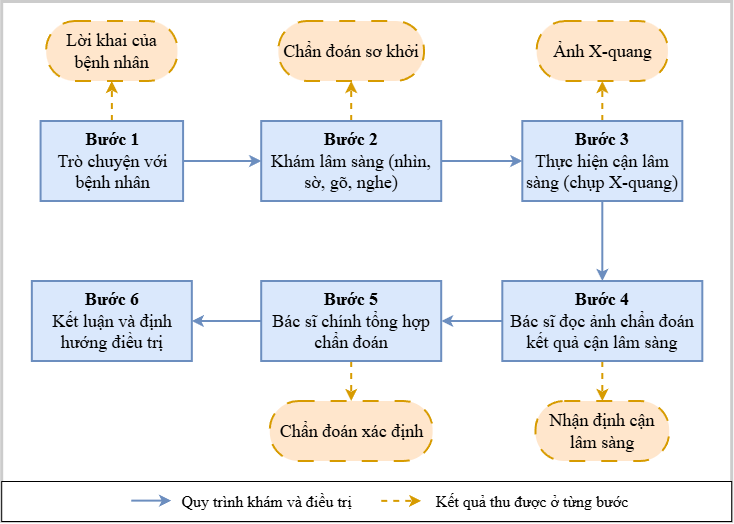
\includegraphics[width=1\linewidth]{images/chapter1/procedure.png}
    \caption{Sơ đồ quy trình khám chữa bệnh lý xương thực tế (các khối xanh) và các kết quả thu được ở từng bước (các khối cam)}
    \label{fig:procedure}
\end{figure}

Thực tiễn dữ liệu thu thập được từ thực tế phục vụ cho việc huấn luyện các mô hình trên còn đưa ra một số hạn chế cần được xử lý liên quan đến mất cân bằng dữ liệu giữa các lớp và việc mô hình cần được xem xét thêm về chi phí thích nghi, hay trường ca bệnh mới chưa từng xuất hiện và khả năng truy vết nguồn thông tin ảnh hưởng đến dự đoán phục vụ cho việc giải thích kết quả hệ thống.

Từ các vấn đề trên, khóa luận đặt ra nhu cầu xây dựng một hệ thống phân lớp X-quang xương đa phương thức có khả năng tận dụng hai nguồn thông tin hình ảnh và văn bản tương tác trực tiếp trước khi phân lớp. Bên cạnh hiệu năng dự đoán, hệ thống cần được đánh giá về sự đánh đổi tài nguyên, khả năng cảnh báo dữ liệu ngoài phân phối và mức độ phụ thuộc của dự đoán vào từng nguồn thông tin. Đây là động lực chính dẫn đến việc đề xuất hệ thống đặt tên XBone-Net trong khóa luận.

\subsection{Vị trí hệ thống trong quy trình khám chữa bệnh lý xương}

Hệ thống được đề xuất trong khóa luận được thiết kế để hỗ trợ bước phân tích ảnh bằng cách khai thác đồng thời ảnh X-quang và dữ liệu văn bản đi kèm để dự đoán lớp bệnh lý, như thể hiện ở Hình~\ref{fig:procedureXbone}. Trên bộ dữ liệu CTCH, văn bản đầu vào là bệnh sử có sẵn trong bệnh án; trong khi đó, BTXRD không cung cấp bệnh sử tự do nên sử dụng văn bản lâm sàng được sinh ngoại tuyến từ siêu dữ liệu. Hai kịch bản được phân tích riêng vì không có mức độ xác thực lâm sàng và mối quan hệ với nhãn tương đương nhau; do đó, kết quả với văn bản tổng hợp không được diễn giải như bằng chứng tương đương với bệnh sử tự nhiên.

\begin{figure}[H]
\centering
    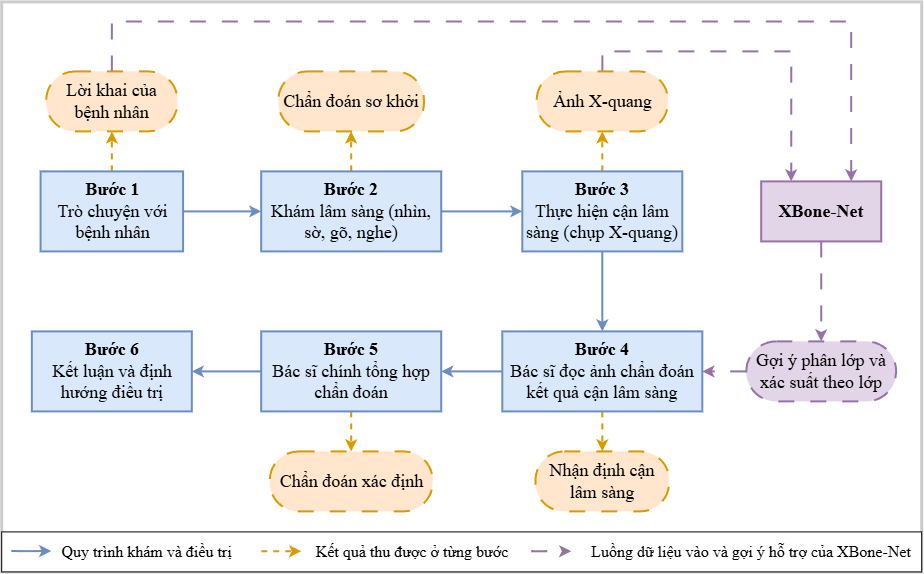
\includegraphics[width=1\linewidth]{images/chapter1/procedureXbone.png}
    \caption{Sơ đồ tích hợp hệ thống hỗ trợ phân tích (các khối tím) vào quy trình khám chữa bệnh lý xương thực tế (các khối xanh) và các kết quả thu được ở từng bước (các khối cam)}
    \label{fig:procedureXbone}
\end{figure}

Khóa luận xem hệ thống trí tuệ nhân tạo là công cụ hỗ trợ phân tích, không thay thế bác sĩ hay tự động hóa quyết định chẩn đoán. Vì vậy, ngoài kết quả phân lớp, nghiên cứu còn khảo sát tín hiệu cảnh báo dữ liệu ngoài phân phối và các bản đồ quy đóng nhằm hỗ trợ phân tích hành vi của mô hình. Các đầu ra này được xem là công cụ đánh giá và truy vết mô hình, chưa phải cơ chế bảo đảm an toàn hay bằng chứng xác nhận vị trí tổn thương trong thực hành lâm sàng.

\section{Giới thiệu bài toán}
\label{sec:ch1_problem_def}

Bài toán được nghiên cứu trong đề tài là bài toán phân lớp đa lớp ảnh X-quang sử dụng học sâu đa phương thức. Mục tiêu của hệ thống là dự đoán các loại bệnh hoặc tổn thương dựa đồng thời vào ảnh X-quang và văn bản đi kèm.
\subsection{Đầu vào}
Hệ thống nhận vào các nguồn dữ liệu sau:
\begin{itemize}
    \item \textbf{Ảnh X-quang của bệnh nhân:}
    \[ x^{\mathrm{img}} \in \mathbb{R}^{H \times W \times C} \] 

    Với $H, W$ là chiều cao và chiều rộng ảnh, $C$ là số kênh màu của ảnh.

    \item \textbf{Văn bản đi kèm:} bệnh sử lâm sàng hoặc văn bản lâm sàng được sinh từ siêu dữ liệu.
    \[ x^{\mathrm{txt}} = (w_1, w_2, \ldots, w_T) \] 

    Với $w_t$ là đơn vị từ ngữ tại vị trí thứ $t$ trong văn bản, $T$ là số lượng đơn vị từ ngữ trong văn bản.

    \item \textbf{Tập nhãn được định nghĩa trước:}
    \[ \mathcal{Y} = \{y_1, y_2, \ldots, y_K\} \] với $K$ là số lớp bệnh cần phân lớp.
\end{itemize}
\subsection{Đầu ra}

Hệ thống sinh ra ba đầu ra chính:

\begin{itemize}
\item \textbf{Cảnh báo dữ liệu ngoài phân phối:}
    \[
        \omega_{\mathrm{OOD}}
        =
        \begin{cases}
            1,
            & \text{nếu }
            s_{\mathrm{OOD}}\left(
                x^{\mathrm{img}},x^{\mathrm{txt}}
            \right) > \tau_{\mathrm{alert}}, \\[4pt]
            0,
            & \text{ngược lại},
        \end{cases}
    \]
Với $s_{\mathrm{OOD}}\left(x^{\mathrm{img}},x^{\mathrm{txt}}\right)$ là điểm bất thường đa phương thức của mẫu đầu vào, $\tau_{\mathrm{alert}}$ là ngưỡng cảnh báo được hiệu chỉnh trước trên tập xác thực và $\omega_{\mathrm{OOD}}=1$ biểu thị rằng hệ thống phát cảnh báo. Cảnh báo này không tự khẳng định mẫu chắc chắn nằm ngoài phân phối.

\item \textbf{Nhãn dự đoán cuối cùng:}
    \[
        \hat{y}
        =
        \operatorname*{arg\,max}_{y_k \in \mathcal{Y}}
        p\left(
        y_k \mid x^{\mathrm{img}},x^{\mathrm{txt}}
        \right),
    \]
Với $p\left(y_k \mid x^{\mathrm{img}},x^{\mathrm{txt}}\right)$ là xác suất dự đoán của lớp $y_k$.

\item \textbf{Thông tin hỗ trợ giải thích:}
Hệ thống sinh ra các bản đồ nhiệt đóng góp cho ảnh toàn cục, các vùng ảnh cục bộ và văn bản đi kèm nhằm khảo sát mức độ liên hệ của từng nguồn thông tin với dự đoán của mô hình.
\end{itemize}


\subsection{Các thách thức trong bài toán}
\label{sec:challenges}
Mặc dù các mô hình học sâu đa phương thức đã đạt được nhiều kết quả tích cực, bài toán vẫn tồn tại nhiều thách thức cần được giải quyết:

\begin{itemize}
    \item \textbf{Sự khác biệt giữa dữ liệu tiền huấn luyện và dữ liệu đầu vào thực tế:} Tồn tại sự chênh lệch giữa các bộ dữ liệu đa phương thức hiện có, thường là cặp ảnh X-quang và báo cáo đọc ảnh, so với dữ liệu đầu vào được khảo sát trong khóa luận gồm ảnh X-quang kết hợp với bệnh sử hoặc thông tin lâm sàng ban đầu. Sự khác biệt này có thể hạn chế khả năng chuyển giao trực tiếp của mô hình.    
    \item \textbf{Hạn chế của dữ liệu thực tế:} Dữ liệu y tế thường có số lượng hạn chế gây mất cân bằng giữa các loại bệnh, đặt ra yêu cầu đặc biệt về thiết kế mô hình để tận dụng tối đa thông tin có sẵn và hạn chế ảnh hưởng của mất cân bằng lớp.
    \item \textbf{Sự khác biệt về không gian và ngữ nghĩa giữa dữ liệu hình ảnh và dữ liệu văn bản:} Sự khác biệt này gây khó khăn cho quá trình học biểu diễn chung, yêu cầu một cơ chế dung hợp hiệu quả.
    \item \textbf{Dữ liệu ngoài phân phối:} Các bộ phân lớp chưa được thiết kế để xử lý các trường hợp dữ liệu ngoài phân phối, dẫn đến nguy cơ đưa ra dự đoán không chính xác với độ tin cậy cao đối với những ca bệnh mới chưa từng xuất hiện trong dữ liệu huấn luyện, đặt ra yêu cầu về khả năng tổng quát hóa và thích ứng của mô hình.
    \item \textbf{Khả năng giải thích của mô hình:} Khả năng giải thích của các mô hình vẫn còn hạn chế khiến độ tin cậy của người dùng vào các dự đoán của hệ thống là không cao, gây khó khăn cho việc triển khai trong thực tế lâm sàng.

\end{itemize}

\section{Mục tiêu nghiên cứu}

Đề tài hướng đến xây dựng và đánh giá một hệ thống học sâu đa phương thức phục vụ phân lớp bệnh lý trên ảnh X-quang xương bằng cách kết hợp thông tin hình ảnh và bệnh sử lâm sàng. Hệ thống được nghiên cứu trong điều kiện mất cân bằng lớp, đồng thời được đánh giá về hiệu năng phân lớp, chi phí tính toán, khả năng cảnh báo dữ liệu ngoài phân phối và mức độ giải thích của dự đoán.

Các mục tiêu cụ thể của đề tài bao gồm:
\begin{enumerate}
\item Xây dựng XBone-Net bằng cách thích nghi BiomedCLIP với LoRA, quy trình huấn luyện hai giai đoạn và mô-đun dung hợp ảnh-văn bản cho bài toán phân lớp X-quang xương.

\item Đánh giá hiệu năng phân lớp của XBone-Net so với các mô hình đối chứng trong thiết lập toàn bộ dữ liệu, đồng thời định lượng sự đánh đổi giữa số tham số cập nhật, chi phí huấn luyện và chi phí suy luận.

\item Thực hiện các thí nghiệm loại bỏ và thay thế thành phần để xác định ảnh hưởng của quy trình huấn luyện và cơ chế dung hợp đến hiệu năng phân loại.

\item Đánh giá hai đầu ra hỗ trợ của hệ thống gồm cảnh báo dữ liệu ngoài phân phối bằng các điểm bất thường hậu xử lý và truy vết nguồn phụ thuộc của dự đoán bằng tích phân gradient kết hợp can thiệp đầu vào.
\end{enumerate}

\section{Đối tượng nghiên cứu}

Đối tượng nghiên cứu của đề tài là các mô hình học sâu đa phương thức trong bài toán phân lớp bệnh lý trên ảnh X-quang xương, sử dụng đồng thời thông tin hình ảnh và bệnh sử lâm sàng. Nghiên cứu tập trung vào các nhóm mô hình và thành phần kỹ thuật sau:

\begin{itemize}
\item Các mô hình ngôn ngữ trực quan được tiền huấn luyện trên dữ liệu tổng quát hoặc dữ liệu y khoa, đóng vai trò bộ mã hóa đặc trưng hình ảnh và văn bản.

\item Các phương pháp biểu diễn ảnh X-quang bằng đơn vị toàn cục và chuỗi đơn vị cục bộ từ các biểu diễn mảnh ảnh từ bộ mã hóa thị giác tiền huấn luyện.

\item Các chiến lược dung hợp đa phương thức, bao gồm phép nối đặc trưng và cơ chế chú ý chéo, để kết hợp biểu diễn hình ảnh với thông tin bệnh sử lâm sàng.

\item Các phương pháp tinh chỉnh hiệu quả tham số cho mô hình tiền huấn luyện quy mô lớn, tập trung vào việc giới hạn số tham số cần cập nhật trong quá trình huấn luyện.

\item Đầu phân lớp tuyến tính kết hợp hàm mất mát có trọng số để xử lý bài toán phân lớp đa lớp trên dữ liệu mất cân bằng.

\item Các phương pháp phát hiện dữ liệu ngoài phân phối và trực quan hóa bản đồ tích phân gradient nhằm hỗ trợ đánh giá độ tin cậy và khả năng giải thích của mô hình.

\end{itemize}

\section{Phạm vi nghiên cứu}
Đề tài tập trung vào bài toán phân lớp đa lớp bệnh lý xương trên ảnh X-quang, kết hợp với bệnh sử lâm sàng. Phạm vi cụ thể bao gồm:

\begin{itemize}
  \item \textbf{Dữ liệu:} Nghiên cứu sử dụng bộ dữ liệu BTXRD \cite{Yao2025} gồm 10 lớp bệnh lý xương và bộ dữ liệu CTCH được thu thập từ Bệnh viện Chấn thương Chỉnh hình Thành phố Hồ Chí Minh.
  \item \textbf{Dữ liệu văn bản:} Bộ dữ liệu CTCH sử dụng bệnh sử có sẵn trong bệnh án, gồm lý do vào viện, diễn tiến bệnh và tiền sử. Bộ dữ liệu BTXRD không có bệnh sử tự do nên sử dụng văn bản lâm sàng được sinh ngoại tuyến từ siêu dữ liệu. Vì mẫu câu tổng hợp có phụ thuộc vào các cờ nhóm bệnh, kết quả BTXRD chỉ phản ánh thiết lập văn bản tổng hợp và không được xem là bằng chứng tương đương với bệnh sử lâm sàng tự nhiên.
  \item \textbf{Vai trò hệ thống:} Hệ thống được thiết kế làm công cụ hỗ trợ phân tích ảnh, không thay thế vai trò của bác sĩ trong quá trình ra quyết định.
  \item \textbf{Giới hạn:} Đề tài không tập trung vào các bài toán phát hiện đối tượng, phân đoạn ảnh hay sinh báo cáo y khoa tự động.
\end{itemize}

\section{Câu hỏi nghiên cứu}

Để đạt được các mục tiêu đã đề ra, nghiên cứu tập trung trả lời các câu hỏi sau:

\begin{itemize}
\item \textbf{Câu hỏi nghiên cứu 1:} Trong tác vụ phân loại, XBone-Net đạt mức hiệu năng phân lớp nào so với các mô hình đối chứng, đồng thời đánh đổi như thế nào giữa số tham số cần cập nhật, chi phí huấn luyện và chi phí suy luận?

\item \textbf{Câu hỏi nghiên cứu 2:} Các thành phần do khóa luận lựa chọn cho XBone-Net, gồm quy trình huấn luyện hai pha và cơ chế dung hợp, ảnh hưởng như thế nào đến hiệu năng phân loại của mô hình?

\item \textbf{Câu hỏi nghiên cứu 3:} Điểm cảnh báo hậu xử lý được xây dựng từ không gian biểu diễn của XBone-Net có thể phân biệt dữ liệu CTCH trong phân phối với các bệnh lý gần miền nằm ngoài không gian nhãn ở mức nào, và kết quả khác nhau ra sao giữa XBone-Net, hai biến thể cùng BiomedCLIP tinh chỉnh toàn bộ?

\item \textbf{Câu hỏi nghiên cứu 4:} Tích phân gradient kết hợp với can thiệp đầu vào phản ánh mức phụ thuộc của dự đoán XBone-Net vào thông tin hình ảnh và văn bản như thế nào?

\end{itemize}

\section{Đóng góp chính của đề tài}

Đóng góp cốt lõi của khóa luận là xây dựng và đánh giá XBone-Net, một phương pháp thích nghi BiomedCLIP và tối ưu hóa đặc trung dữ liệu phục vụ cho bài toán phân lớp X-quang xương đa phương thức. Các đóng góp chính gồm:

\begin{enumerate}
    \item \textbf{Đề xuất quy trình tối ưu biểu diễn dữ liệu cho phân loại:} kết hợp LoRA trên hai bộ mã hóa của BiomedCLIP, huấn luyện hai pha và cơ chế chú ý chéo hai chiều để vừa thích nghi biểu diễn với miền X-quang xương, vừa khai thác bổ sung ngữ nghĩa giữa đặc trưng hình ảnh và văn bản trước khi phân lớp. Điều này cũng tạo tiền đề cho hiệu năng phát hiện dữ liệu ngoài phân phối và khả năng giải thích dự đoán.

    \item \textbf{Đánh giá có hệ thống hiệu năng và sự đánh đổi tài nguyên:} thực nghiệm với các mô hình đối chứng và các cấu hình loại bỏ thành phần cho thấy XBone-Net đạt hiệu năng cạnh tranh với các mô hình ngôn ngữ-thị giác tinh chỉnh toàn bộ, trong khi chỉ cập nhật khoảng 4,13\% tổng số tham số và giảm hơn 60\% bộ nhớ GPU cực đại trong huấn luyện; đồng thời khóa luận chỉ ra chi phí đánh đổi về thời gian huấn luyện và suy luận.

    \item \textbf{Bổ sung đánh giá độ tin cậy và khả năng truy vết dự đoán:} xây dựng điểm cảnh báo dữ liệu ngoài phân phối từ không gian biểu diễn đa phương thức và sử dụng tích phân Gradients kết hợp can thiệp đầu vào để khảo sát mức phụ thuộc của dự đoán vào ảnh và văn bản. Hai thành phần này được xem là công cụ hỗ trợ phân tích mô hình, không phải cơ chế bảo đảm an toàn hoặc bằng chứng nhân quả về quyết định lâm sàng.
\end{enumerate}

\section{Bố cục khóa luận}

Khóa luận được tổ chức thành năm chương như sau:

\textbf{Chương 1: Giới thiệu.} Chương này trình bày bối cảnh nghiên cứu, vấn đề đặt ra, mục tiêu, đối tượng, câu hỏi nghiên cứu và các đóng góp chính của đề tài. Nội dung chương đóng vai trò định hướng cho toàn bộ khóa luận.

\textbf{Chương 2: Các công trình nghiên cứu liên quan.} Chương này tổng quan các nghiên cứu về mô hình ngôn ngữ trực quan, phân lớp ảnh X-quang xương, xử lý ảnh độ phân giải cao, dung hợp đa phương thức, tinh chỉnh hiệu quả tham số, phát hiện dữ liệu ngoài phân phối và khả năng giải thích mô hình. Trên cơ sở đó, chương xác định khoảng trống nghiên cứu và định vị phương pháp đề xuất so với các công trình trước.

\textbf{Chương 3: Phương pháp đề xuất.} Chương này mô tả kiến trúc XBone-Net, quy trình xử lý ảnh và văn bản, cơ chế dung hợp hai chiều, đầu phân lớp tuyến tính, các hàm mất mát và chiến lược huấn luyện hai giai đoạn với LoRA. Quy trình phát hiện dữ liệu ngoài phân phối và giải thích dự đoán cũng được trình bày trong chương này.

\textbf{Chương 4: Thực nghiệm và kết quả.} Chương này giới thiệu các bộ dữ liệu, thiết lập thực nghiệm, mô hình đối sánh và các độ đo đánh giá. Các kết quả toàn bộ mẫu, nghiên cứu loại bỏ thành phần, đánh giá hiệu quả tính toán, phát hiện dữ liệu ngoài phân phối và giải thích mô hình được phân tích nhằm làm rõ ưu điểm, hạn chế và sự đánh đổi của phương pháp đề xuất.

\textbf{Chương 5: Kết luận và hướng phát triển.} Chương cuối tổng kết các kết quả đạt được, trả lời các câu hỏi nghiên cứu, chỉ ra những hạn chế còn tồn tại và đề xuất các hướng cải tiến, mở rộng trong tương lai.
